% Created by tikzDevice version 0.7.0 on 2015-04-19 22:32:31
% !TEX encoding = UTF-8 Unicode
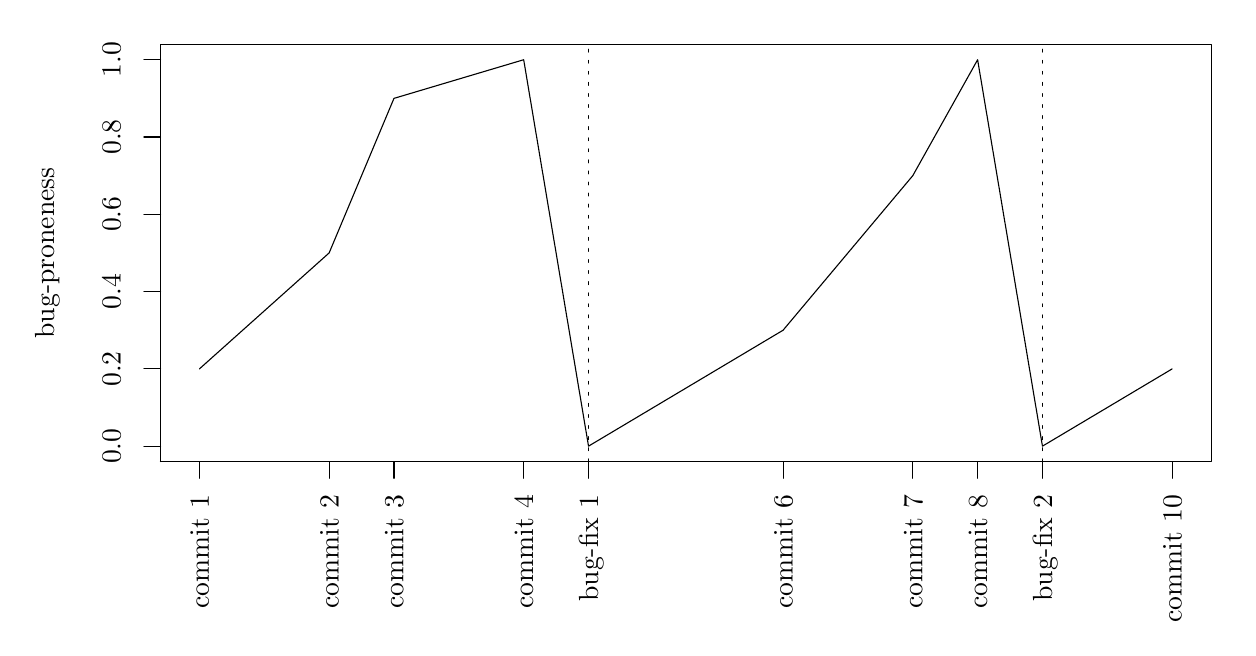
\begin{tikzpicture}[x=1pt,y=1pt]
\definecolor[named]{fillColor}{rgb}{1.00,1.00,1.00}
\path[use as bounding box,fill=fillColor,fill opacity=0.00] (0,0) rectangle (433.62,216.81);
\begin{scope}
\path[clip] ( 48.00, 60.00) rectangle (427.62,210.81);
\definecolor[named]{drawColor}{rgb}{0.00,0.00,0.00}

\path[draw=drawColor,line width= 0.4pt,line join=round,line cap=round] ( 62.06, 93.51) --
	(108.93,135.41) --
	(132.36,191.26) --
	(179.23,205.22) --
	(202.66, 65.59) --
	(272.96,107.48) --
	(319.83,163.33) --
	(343.26,205.22) --
	(366.69, 65.59) --
	(413.56, 93.51);
\end{scope}
\begin{scope}
\path[clip] (  0.00,  0.00) rectangle (433.62,216.81);
\definecolor[named]{drawColor}{rgb}{0.00,0.00,0.00}

\path[draw=drawColor,line width= 0.4pt,line join=round,line cap=round] ( 48.00, 65.59) -- ( 48.00,205.22);

\path[draw=drawColor,line width= 0.4pt,line join=round,line cap=round] ( 48.00, 65.59) -- ( 42.00, 65.59);

\path[draw=drawColor,line width= 0.4pt,line join=round,line cap=round] ( 48.00, 93.51) -- ( 42.00, 93.51);

\path[draw=drawColor,line width= 0.4pt,line join=round,line cap=round] ( 48.00,121.44) -- ( 42.00,121.44);

\path[draw=drawColor,line width= 0.4pt,line join=round,line cap=round] ( 48.00,149.37) -- ( 42.00,149.37);

\path[draw=drawColor,line width= 0.4pt,line join=round,line cap=round] ( 48.00,177.30) -- ( 42.00,177.30);

\path[draw=drawColor,line width= 0.4pt,line join=round,line cap=round] ( 48.00,205.22) -- ( 42.00,205.22);

\node[text=drawColor,rotate= 90.00,anchor=base,inner sep=0pt, outer sep=0pt, scale=  1.00] at ( 33.60, 65.59) {0.0};

\node[text=drawColor,rotate= 90.00,anchor=base,inner sep=0pt, outer sep=0pt, scale=  1.00] at ( 33.60, 93.51) {0.2};

\node[text=drawColor,rotate= 90.00,anchor=base,inner sep=0pt, outer sep=0pt, scale=  1.00] at ( 33.60,121.44) {0.4};

\node[text=drawColor,rotate= 90.00,anchor=base,inner sep=0pt, outer sep=0pt, scale=  1.00] at ( 33.60,149.37) {0.6};

\node[text=drawColor,rotate= 90.00,anchor=base,inner sep=0pt, outer sep=0pt, scale=  1.00] at ( 33.60,177.30) {0.8};

\node[text=drawColor,rotate= 90.00,anchor=base,inner sep=0pt, outer sep=0pt, scale=  1.00] at ( 33.60,205.22) {1.0};

\path[draw=drawColor,line width= 0.4pt,line join=round,line cap=round] ( 48.00, 60.00) --
	(427.62, 60.00) --
	(427.62,210.81) --
	( 48.00,210.81) --
	( 48.00, 60.00);
\end{scope}
\begin{scope}
\path[clip] (  0.00,  0.00) rectangle (433.62,216.81);
\definecolor[named]{drawColor}{rgb}{0.00,0.00,0.00}

\node[text=drawColor,rotate= 90.00,anchor=base,inner sep=0pt, outer sep=0pt, scale=  1.00] at (  9.60,135.41) {bug-proneness};
\end{scope}
\begin{scope}
\path[clip] (  0.00,  0.00) rectangle (433.62,216.81);
\definecolor[named]{drawColor}{rgb}{0.00,0.00,0.00}

\path[draw=drawColor,line width= 0.4pt,line join=round,line cap=round] ( 62.06, 60.00) -- (413.56, 60.00);

\path[draw=drawColor,line width= 0.4pt,line join=round,line cap=round] ( 62.06, 60.00) -- ( 62.06, 54.00);

\path[draw=drawColor,line width= 0.4pt,line join=round,line cap=round] (108.93, 60.00) -- (108.93, 54.00);

\path[draw=drawColor,line width= 0.4pt,line join=round,line cap=round] (132.36, 60.00) -- (132.36, 54.00);

\path[draw=drawColor,line width= 0.4pt,line join=round,line cap=round] (179.23, 60.00) -- (179.23, 54.00);

\path[draw=drawColor,line width= 0.4pt,line join=round,line cap=round] (202.66, 60.00) -- (202.66, 54.00);

\path[draw=drawColor,line width= 0.4pt,line join=round,line cap=round] (272.96, 60.00) -- (272.96, 54.00);

\path[draw=drawColor,line width= 0.4pt,line join=round,line cap=round] (319.83, 60.00) -- (319.83, 54.00);

\path[draw=drawColor,line width= 0.4pt,line join=round,line cap=round] (343.26, 60.00) -- (343.26, 54.00);

\path[draw=drawColor,line width= 0.4pt,line join=round,line cap=round] (366.69, 60.00) -- (366.69, 54.00);

\path[draw=drawColor,line width= 0.4pt,line join=round,line cap=round] (413.56, 60.00) -- (413.56, 54.00);

\node[text=drawColor,rotate= 90.00,anchor=base east,inner sep=0pt, outer sep=0pt, scale=  1.00] at ( 65.50, 48.00) {commit 1};

\node[text=drawColor,rotate= 90.00,anchor=base east,inner sep=0pt, outer sep=0pt, scale=  1.00] at (112.37, 48.00) {commit 2};

\node[text=drawColor,rotate= 90.00,anchor=base east,inner sep=0pt, outer sep=0pt, scale=  1.00] at (135.80, 48.00) {commit 3};

\node[text=drawColor,rotate= 90.00,anchor=base east,inner sep=0pt, outer sep=0pt, scale=  1.00] at (182.67, 48.00) {commit 4};

\node[text=drawColor,rotate= 90.00,anchor=base east,inner sep=0pt, outer sep=0pt, scale=  1.00] at (206.10, 48.00) {bug-fix 1};

\node[text=drawColor,rotate= 90.00,anchor=base east,inner sep=0pt, outer sep=0pt, scale=  1.00] at (276.40, 48.00) {commit 6};

\node[text=drawColor,rotate= 90.00,anchor=base east,inner sep=0pt, outer sep=0pt, scale=  1.00] at (323.27, 48.00) {commit 7};

\node[text=drawColor,rotate= 90.00,anchor=base east,inner sep=0pt, outer sep=0pt, scale=  1.00] at (346.70, 48.00) {commit 8};

\node[text=drawColor,rotate= 90.00,anchor=base east,inner sep=0pt, outer sep=0pt, scale=  1.00] at (370.14, 48.00) {bug-fix 2};

\node[text=drawColor,rotate= 90.00,anchor=base east,inner sep=0pt, outer sep=0pt, scale=  1.00] at (417.00, 48.00) {commit 10};
\end{scope}
\begin{scope}
\path[clip] ( 48.00, 60.00) rectangle (427.62,210.81);
\definecolor[named]{drawColor}{rgb}{0.00,0.00,0.00}

\path[draw=drawColor,line width= 0.4pt,dash pattern=on 1pt off 3pt ,line join=round,line cap=round] (202.66, 60.00) -- (202.66,210.81);

\path[draw=drawColor,line width= 0.4pt,dash pattern=on 1pt off 3pt ,line join=round,line cap=round] (366.69, 60.00) -- (366.69,210.81);
\end{scope}
\end{tikzpicture}
